\chapter{Methodology}\label{chapter:methodology}


% NOTE: add HMM as baseline

This work aims to construct a graph neural network-based architecture for predicting, analyzing, and detecting any potentially abnormal behavior regarding the driver during the whole driving process. In particular, The model extracts a description graph, the so-called scene graph, of the driver from the video filmed inside the vehicle and trains itself with these data to learn for future behavior prediction. The result will be used to compare and detect any abnormal behavior. Here we would lay most emphasis on the construction of the training model. To make precious anomaly detection we aim to predict not only if there is a behavior between humans and a specific kind of object but the type of behavior as well, which will cause several adaptions based on existing model \textit{JODIE}. 

This chapter will follow the pipeline of the whole work, as shown in figure \ref{fig:pipeline}. Progressively we would introduce the scene graph generation, the model architecture, and the training process. 

\begin{figure}
    \centering
    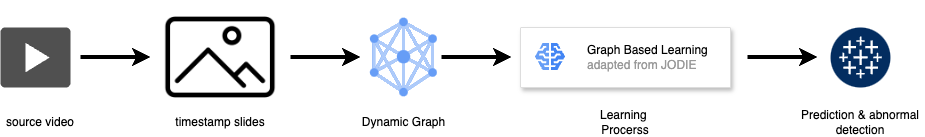
\includegraphics[width=\linewidth]{figures/04_pipeline.png}
    \caption{Pipeline of the whole work}
    \label{fig:pipeline}
\end{figure}


\section{Scene graph generation}

The \textit{Drive \& Act} dataset comprises 12 hours of video data segmented into 29 lengthy sequences. For each sequence, we aim to generate a unique dynamic graph that temporally represents both the participant's actions and the relationships between objects observed in the video. This process involves several key steps.


First, by sliding through the video at intervals of $1/15$ per second, we obtain a series of images. Theoretically, each image could yield a corresponding graph with the use of an object detection model \cite{tang2020unbiased}. Given that our objective is to predict driver behavior, we concentrate on the driver and the specific objects with which they interact. Consequently, we opt for a streamlined approach by directly extracting data from hierarchical labels within the dataset. Table \ref{tab:hierarchical_labels_task}and table \ref{tab:hierarchical_labels_object} provide an overview of the hierarchical labels. The former provides the concrete activity descriptions of the driver in specific time frames, while the latter outlines the objects the driver interacts with, along with the corresponding locations where these interactions occur.

\clearpage

\begin{longtable}{ccccc}
    \toprule
    \textbf{file\_id} & \textbf{frame\_start} & \textbf{frame\_end} & \textbf{activity} & \textbf{chunk\_id} \\
    \midrule
    vp1/run1b.kinect\_color & 40 & 58 & standing\_by\_the\_door & 0 \\
    vp1/run1b.kinect\_color & 58 & 82 & closing\_door\_outside & 0 \\
    vp1/run1b.kinect\_color & 83 & 102 & standing\_by\_the\_door & 0 \\
    vp1/run1b.kinect\_color & 102 & 130 & opening\_door\_outside & 0 \\
    vp1/run1b.kinect\_color & 130 & 156 & entering\_car & 0 \\
    vp1/run1b.kinect\_color & 156 & 174 & closing\_door\_inside & 0 \\
    \bottomrule
    \caption{Example of the  task level hierarchical labels Reproduced from\cite{9009583}}
    \label{tab:hierarchical_labels_task}
\end{longtable}

\begin{table}[h!]
    \centering
    \begin{tabular}{ccccc}
    \toprule
    \textbf{Start Time} & \textbf{End Time} & \textbf{Action}         & \textbf{Object}               & \textbf{Location}           \\ 
    \midrule
    175                 & 188               & reaching\_for           & seatbelt                     & left\_backseat              \\ 
    \midrule
    189                 & 208               & retracting\_from        & seatbelt                     & left\_backseat              \\ 
    \midrule
    208                 & 230               & interacting             & seatbelt                     & no\_location                \\ 
    \midrule
    240                 & 258               & reaching\_for           & multimedia\_display          & center\_console\_front      \\ 
    \midrule
    3011                & 3031              & reaching\_for           & automation\_button           & center\_console\_back       \\ 
    \midrule
    3031                & 3056              & retracting\_from        & no\_object                   & center\_console\_back       \\ 
    \midrule
    3115                & 3144              & reaching\_for           & multimedia\_display          & center\_console\_front      \\ 
    \midrule
    3144                & 3156              & retracting\_from        & no\_object                   & center\_console\_front      \\ 
    \midrule
    3311                & 3357              & reaching\_for           & no\_object                   & right\_backseat             \\ 
    \bottomrule
    \end{tabular}
    \caption{Example of the  object level hierarchical labels Reproduced from\cite{9009583}}
    \label{tab:hierarchical_labels_object}
    \end{table}
    


However, these tables alone are insufficient for generating graphs, as object detection at each individual timestamp is required to ensure data completeness. In other words, the row \textit{start time} and \textit{end time} will be replaced by \textit{Timestamp}. To address this, we construct the dynamic graph by processing each timestamp sequentially. Specifically, the participant is designated as the node $u$, and all relevant objects are represented as nodes $i$. By analyzing interactions at each timestamp, edges are added between the participant node and the corresponding object nodes to represent the associated actions. Additionally, the features of the edges are enriched with the location where each action occurs. The graph is iteratively updated with each subsequent timestamp, ultimately resulting in a dynamic graph that captures the temporal evolution of interactions.
    


Another key consideration in graph generation is the classification of activity labels. The raw dataset contains 39 distinct behaviors, which would be computationally intensive and overly too trivial to label directly. To address this, we employ \textit{BART}, a denoising autoencoder designed for pretraining sequence-to-sequence models, to cluster these behaviors into four categories. This classification is based on two key questions: whether the behavior is related to driving and whether it implies any potential risk, as the ultimate goal is to identify and flag abnormal behaviors. The resulting behavior classifications are presented in Table \ref{tab:Behavior classification}.

\begin{figure}[h]
    \centering
    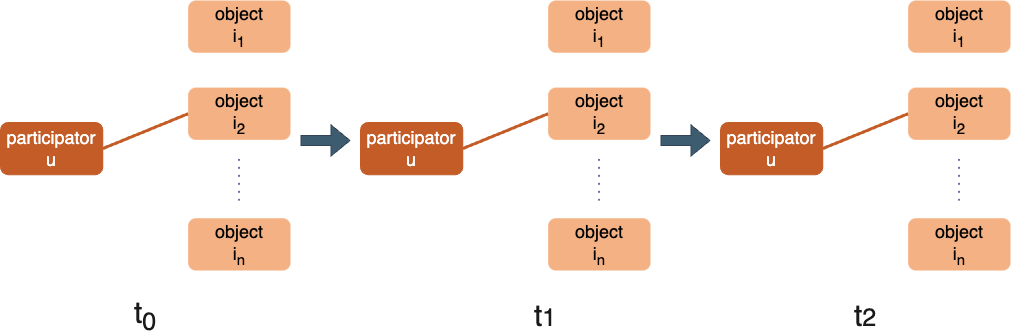
\includegraphics[width=\linewidth]{figures/04_DynamicGraph.png}
    \caption{Dynamic Graph Generation for Driver Behavior Recognition}
    \label{fig:DynamicGraph}
\end{figure}


% \clearpage

\begin{table}[h]
    \centering
    \begin{tabular}{ccp{10cm}}
        \toprule
        \textbf{No.} & \textbf{State} & \textbf{Behaviors} \\
        \midrule
        1 & \textbf{Driving concerned behaviors} & standing by the door, closing door outside, opening door outside, entering car, closing door inside, fastening seat belt, moving towards door, unfastening seat belt, opening door inside, exiting car \\
        \midrule
        2 & \textbf{Independent behaviors} & sitting still, looking or moving around (e.g. searching), looking back left shoulder, looking back right shoulder \\
        \midrule
        3 & \textbf{Eat or drink concerned behaviors} & preparing food, eating, opening bottle, drinking, closing bottle \\
        \midrule
        4 & \textbf{Other object concerned behaviors} & using multimedia display, sitting still, using multimedia display, pressing automation button, fetching an object, opening laptop, working on laptop, interacting with phone, closing laptop, placing an object, putting on jacket, taking off sunglasses, putting on sunglasses, reading newspaper, writing, talking on phone, reading magazine, taking off jacket, opening backpack, closing backpack, putting laptop into backpack, taking laptop from backpack \\
        \bottomrule
    \end{tabular}
    \caption{Behavior classification}
    \label{tab:Behavior classification}
\end{table}



Through the processes outlined above, all dynamic graphs have been successfully generated, as illustrated in Figure \ref{fig:DynamicGraph}. To streamline subsequent learning steps, these graphs are stored in a tabular format, as shown in Table \ref{tab:dynamic_graph_storage}.



\begin{table}[h]
    \centering
    \begin{tabular}{ccccc}
        \toprule
        \textbf{u} & \textbf{i} & \textbf{timestamp} & \textbf{state label} & \textbf{feature} \\
        \midrule
        1 & 2 & 127 & 0 & 0.27 \\
        \bottomrule
    \end{tabular}
    \caption{Storage of dynamic graph}
    \label{tab:dynamic_graph_storage}
\end{table}

As illustration of heads of this table is as following:

\begin{description}
    \item[u] The action initiator or generator, in our work typically representing the participant or driver.
    \item[i] The object or target that is acted upon or influenced by the action.
    \item[timestamp] The specific moment or time frame at which the action or interaction occurs.
    \item[stable label] A stable vector that characterizes the consistent attributes or categorical label associated with the edge.
    \item[feature] A weight vector representing the proportion of occurrences for a particular attribute (in this case, the location column), reflecting the relative frequency or appearance percentage of this attribute over time.
\end{description}


% we classify and label the behavior with LLM

\section{Baseline: Hidden Markov Model (HMM)}


The Hidden Markov Model (HMM) is a suitable baseline for our driver behavior prediction task due to its effectiveness in modeling temporal sequences with underlying hidden states, allowing it to capture the evolving patterns of driver behavior over time. HMMs provide a probabilistic framework that handles uncertainty in sequential data, making them a widely adopted baseline for tasks involving sequence prediction, including applications in graph neural network (GNN) models. In our work, this baseline serves as a foundation for comparison, particularly given that our hybrid model does not align directly with more complex modern models, which may lack sufficient parallels for a direct comparison.

To perform the prediction task, we first extract the temporal sequence from the dynamic graph data. In this context, the state represents a classification of similar behaviors observed within the dataset, while the features encapsulate consequential representations that may influence future observations. Thus, we set the value \textit{state label} as the observation sequence and the \textit{feature} as the hidden state, see in figure\ref{fig:HMMmodel}.

With the help of the library \textit{hmmlearn}, we can train the model with the extracted data and predict the state of the next timestamp. Comparing the predicted state with the actual state, we can evaluate the performance of HMM. And the result will be used as a baseline for the following models.
\begin{figure}[h]
    \centering
    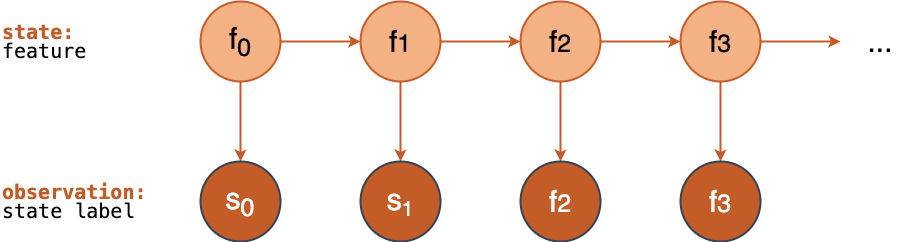
\includegraphics[width=0.8\linewidth]{figures/04_HMMmodel.png}
    \caption{HMM Model Architecture}
    \label{fig:HMMmodel}
\end{figure}


\section{Training Model Architecture}

\subsection{Introduction to JODIE}
% what is JODIE
As is mentioned in chapter \ref{chapter:relatedwork}, the model \textit{JODIE} is a coupled recurrent neural network model that learns the embedding trajectories of users and items. Before we start our own contribution to the model, some introduction to the original model is necessary.

The model \textit{JODIE} is aimed at learning the embedding trajectories of users, denoted as $\mathbf{u(t)} \in \mathbb{R} ^n$ for each $u \in \mathcal{U}$ and item, denoted as $\mathbf{i(t)} \in \mathbb{R} ^n$ for each $i \in \mathcal{I} $, over a time interval $\forall t \in [0,T] $. These embeddings are derived from an ordered sequence of temporal user-item interactions $S_r=(u_r,i_r,t_r,\mathbb{f}_r)$, which indicates that an interaction $S_r$ involving a user $u_r \in \mathcal{U} $ and an item $i_r \in \mathcal{I} $ at time $t_r \in \mathbb{R} ^+$, in the period $0 < t_1 < t_2< \cdots  < T$. In our study, the \textit{user} corresponds to the driver, and the \textit{item} to the object of which the action will take place. The process of interaction thus represents the driver’s behavior toward the object over time.

To encode both long-term stationary properties and the dynamic evolution of user-item interactions, the embedding contains \textbf{static and dynamic embeddings}. Static embeddings $\mathbf{\overline{u} } \in \mathbb{R} ^d \ \forall u \in \mathcal{U}$ and $\mathbf{\overline{i} } \in \mathbb{R} ^d \ \forall i \in \mathcal{I}$ keep constant over time, with one-hot vectors representation similar in LSTM\cite{zhu2017next} and TimeAware-LSTM\cite{baytas2017patient}. In contrast, the dynamic embeddings are designed to evolve with each interaction: each user and item is associated with a dynamic embedding, $\mathbf{u(t)}$ and $\mathbf{i(t)}$, respectively. These dynamic embeddings change over time, producing what is referred to as an \textit{embedding trajectory} that reflects the historical sequence of interactions.


\subsection{Core Components of JODIE}

The model could be separated into two parts: the \textbf{update operation} and the \textbf{projection operation}. The former update the embeddings of the user and the item, while the latter uses the previous observed state and the elapsed time to predict the future embedding of the user. The figure \ref{fig:JODIE} illustrates the architecture of the model.

In the \textbf{update operation}, the interaction $S=(u,i,t,f)$ between a user $u$ and item $i$ at time $t$ is used to generated their dynamic embeddings $\mathbf{u(t)}$ and $\mathbf{i(t)}$. Two recurrent neural networks RNNs are involved in this process, named $RNN_U$ and  $RNN_I$. They recursively update the embeddings of the user and the item. This structure offers significant advantages over traditional one-hot vector representations, as the dynamic embedding reflects the item’s current state. This leads to more meaningful user embeddings and streamlines the training process. The dynamic embeddings are updated as follows:

\[ \mathbf{u(t)}=\sigma(W_1^u\mathbf{u(t^-)}+W_2^u\mathbf{i(t^-)}+W_3^u \mathbf{f}  + W^u_4 \Delta _u)\]
\[
\mathbf{i(t)} = \sigma (W_1^i \mathbf{i(t^-)} + W_2^i \mathbf{u(t^-)} + W_3^i \mathbf{f} + W_4^i \Delta_i)
\]



where $\Delta _u$ denotes the time since the last interaction of user $u$ and $\Delta _i$ denotes the time since the last interaction of item $i$. $\mathbf{f}$ is the representation of the interaction, in another word, the feature vector. All the matrices $W_1^u \dots W_4^u$ and $W_1^i \dots W_4^i$ are parameters belong to $RNN_U$ and $RNN_I$ respectably, they will be trained to predict the embedding of the item at $u$'s next interaction. $\sigma$ is a sigmoid function to introduce non-linearity.

In the \textbf{projection operation}, the future trajectory of the user embedding is predicted. This projection occurs at a specified time interval, $\delta$ after the last interaction at time $t$, when the user's embedding is update to $u(t+\Delta)$. 
In order to effectively embed time-sequence data, the method \textit{LatentCross}\cite{10.1145/3159652.3159727} is introduced, which creates a temporal attention vector. Firstly, $\Delta$ needs to convert into a time-context vector $\mathbf{w} \in \mathbb{R} ^n$ using a linear layer $\mathbf{w} =W_p \Delta$, and $W_p$ is a learnable vector initialized from a zero-mean Gaussian distribution. The projected embedding is then derived by taking the element-wise product of the time-context vector and the previous embedding as follows:

\[ \hat{u}(t+ \Delta) = (1+\mathbf{w})*\mathbf{u(t)} \]

Here the vector $1+\mathbf{w}$ is a temporal attention to scale the past user embedding. According to the original \textit{LatentCross} work, a linear layer is optimal for projecting the embedding, as introducing non-linearity can distort the embedding. Consequently, we retain this linear layer in our implementation.

\begin{figure}[h]
    \centering
    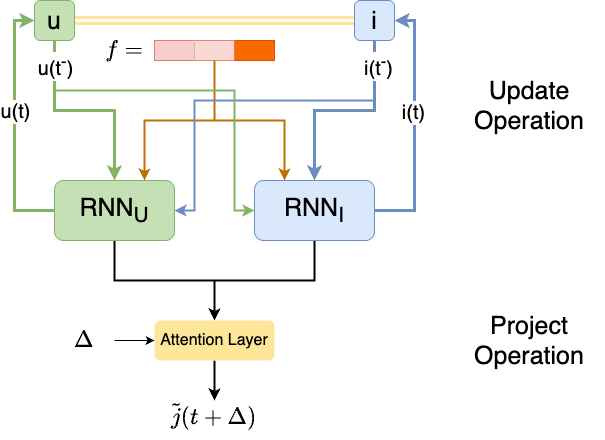
\includegraphics[width=\linewidth]{figures/04_JODIE.png}
    \caption{JODIE Model Architecture}
    \label{fig:JODIE}
\end{figure}



\subsection{Training Process of JODIE}

Let $u$ interact with item $i$ at time $j$ and then with item $j$ at time $t + \Delta$. Right before $t + \Delta$, can we predict which item u will interact with? We use this task to train the update and projection operations in JODIE. We train JODIE to make this prediction using u’s projected embedding $ \hat{u}(t+ \Delta)$. Rather than computing the interaction probability between each user $u$ and item $i$, \textit{JODIE} directly outputs an item embedding vector $\tilde{j}(t + \Delta)$. This approach allows \textit{JODIE} to make predictions with a single forward pass of the prediction layer, significantly reducing computational demands during inference by bypassing additional neural network passes. Using Locality Sensitive Hashing (LSH) techniques \cite{rajaraman2011mining}, we can then retrieve the item with the closest embedding in near-constant time.

Thus, \textit{J} is trained to minimize the $L_2$ difference between the predicted item embedding $\tilde{j}(t + \Delta)$ and the real item embedding $[\overline{j}, j(t + \Delta^-)]$. The latter is a concatencation of the static embedding $\overline{j}$ and the dynamic embedding $j(t + \Delta^-)$ that immediately before time $t+\Delta$. The loss function is defined as follows:
\[ \| \tilde{j}(t + \Delta) - [\overline{j}, j(t + \Delta^-)] \|_2 \]

As for the prediction, it is mad using a fully connected linear layer as follows:

\[\tilde{j}(t+\Delta)=W_1\mathbf{\hat{u}(t+\Delta)}+W_2\mathbf{\bar{u}}+W_3\mathbf{i(t+\Delta ^-)}+W_4\mathbf{\bar{i}}+B\]

This prediction leverages the projected user embedding, $\hat{u}(t+\delta)$ nd the embedding of the item from $u$'s most recent interaction immediately before $t+\Delta$,denoted as $i(t+\Delta ^-)$. The inclusion of $i(t+\Delta ^-)$ is crucial, as users frequently interact with the same item consecutively (i.e.,$i=j$) , and incorporating the item embedding simplifies the prediction. This consideration is especially important in our work, where the scenario is based on the assumption that the driver interacts with the same object throughout the driving process. The matrices $W_1,W_2,W_3,W_4$ and $B$ are learnable parameters, and the loss function is defined as the mean squared error between the predicted and actual item embeddings. Additionally, static embeddings are included to capture long-term properties of both the user and the item, ensuring a comprehensive prediction.

Finally, the total loss function is calculated as following:

\begin{equation}
    \text{Loss} = \sum_{(u, i, t, f) \in S} \left\| \tilde{j}(t) - \left[ \bar{i}, i(t^-) \right] \right\|_2 
    + \lambda_U \left\| \mathbf{u}(t) - \mathbf{u}(t^-) \right\|_2 
    + \lambda_I \left\| \mathbf{i}(t) - \mathbf{i}(t^-) \right\|_2
    \end{equation}


The first term minimizes the  $L_2$ distance between the predicted item embedding and the ground truth item embedding at each interaction. The last two terms serve as regularization, preventing excessive variation in consecutive dynamic embeddings of the user and item. Scaling parameters  $\lambda_U$ and $\lambda_U$ ensure the losses are within the same range. Notably, negative sampling is not used during training to avoid overfitting.


In the original paper, the authors also propose an extension of JODIE for prediction tasks with categorical outputs rather than binary ones. In such cases, additional training labels are required, and the prediction function is redefined as $\mathbb{R} ^{n+d}\rightarrow C$ enabling label prediction using the user embedding after an interaction. Here, the cross-entropy loss is calculated for categorical labels and incorporated into the overall loss function with an additional scaling parameter. The following section will discuss how this adaptation is implemented in our work.




\subsection{Adapting JODIE to Enhance Interaction State Prediction}
\begin{figure}[h]
    \centering
    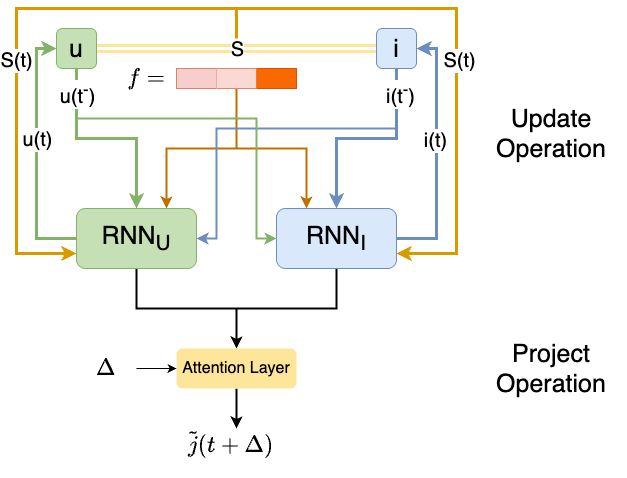
\includegraphics[width=\linewidth]{figures/04_JODIE_with_state.png}
    \caption{JODIE Model Architecture with State Prediction}
    \label{fig:JODIE_with_state}
\end{figure}


Returning to our initial goal, the primary objective is to predict the behavior of the driver. Therefore, it is essential to account for both the object the driver interacts with and the driver’s behavior toward that object. In the original \textit{JODIE} model, only the object is predicted as the node to which the edge will connect in the subsequent timestamp. However, in our approach, the behavior is represented as the classification of each edge connecting the user and item nodes in the dynamic graph, referred to as the \textit{state} of each edge. Incorporating the \textit{state} into the \textbf{embedding space} and modifying the \textbf{loss function} accordingly enables the prediction of behavior. The proposed adaptations are illustrated in Figure \ref{fig:JODIE_with_state}. To accomplish this, we explicitly add the interaction state into the embeddings of both the user and the item: 


\[ \mathbf{u(t)} = \sigma (W_1^u \mathbf{u(t^-)} + W_2^u \mathbf{i(t^-)} + W_3^u \mathbf{f} + W^u_4s+W^u_5\Delta _u) \]

\[ \mathbf{i(t)} = \sigma (W_1^i \mathbf{i(t^-)} + W_2^i \mathbf{u(t^-)} + W_3^i \mathbf{f} + W^i_4s+W^u_5 \Delta _i) \]


Similar to other matrices, $W^u_4$ and $W^i_4$ are also learnable parameters. Their values, denoted as $s$, have been enumerated in the previous steps and undergo a linear transformation before being incorporated into the embedding space. This adaptation enhances the representation of the embedding spaces for both the user $u$ and the item $i$, providing additional information crucial for predicting the behavior state in future interactions. This modification is then integrated into the prediction function, which is updated as follows:

\[ \tilde{j}(t+\Delta)=W_1\hat{u}(t+\delta)+W_2\bar{u}+W_3i(t+\Delta ^-)+W_4\bar{i}+W_5s+B \]

To meet the final goal of predicting the behavior state, the loss function's output  of potential edge appearance should be converted from a binary classification(if the user will interact with the item) to a multi-class classification (either the user won't interact with this item, or one kind of interaction would be taken place here). In a mathematic representation, the domain of the output would convert from a binary set $\{0,1\}$ to a set of $n$ classes ${0,s_1,s_2,s_3,s_4}$. In this case, the cross-entropy loss function is used to calculate the difference between the predicted and actual behavior states. 



Several steps are required to adapt the model for this task:
\begin{description}
    \item[update the prediction Mechanism]
    In the original model, predictions are made using a fully connected linear layer. However, in our case, the requirement is to determine the correct relationship between two nodes, $u \in \mathcal{U} $ and $i \in \mathcal{I} $. This relationship falls into one of five categories: no connection, or connections labeled with $s_1$ through $s_4$. Consequently, the embedding space needs to be transformed into a 5-dimensional vector. To extract the predicted probability $p(t)$, the output of the linear layer is passed through a softmax function, obtaining a probability distribution over the behavior states.
    \[ p(t)=softmax(W \tilde{j}(t) + b)\]

    Here $W$ is a learnable parameter matrix and $b$ is a bias term, the probability distribution $p \in \mathbb{R} ^{5 \times n}$ to match the dimension of the output.
    \item[Cross-Entropy loss] 
    
    The Cross-Entropy loss for a single interaction is expressed as:
    \[ \text{Loss}_{CE} = -\sum_{k=1}^{5} y_k \log p_k(t) \]
    where $y_k$ is the ground truth label of the behavior state, and $p_k(t)$ is the predicted probability of the behavior state. The total loss is the sum of the losses for all interactions in the dataset.
    
    
    \item[Integrate into the overall loss function] 
    
    Incorporating this into the overall loss function, the updated objective becomes:

    \begin{equation}
        \text{Loss} = \sum_{(u, i, t, f) \in S} \text{Loss}_{CE}(t)
        + \lambda_U \left\| \mathbf{u}(t) - \mathbf{u}(t^-) \right\|_2 
        + \lambda_I \left\| \mathbf{i}(t) - \mathbf{i}(t^-) \right\|_2
        \end{equation}
    where $\sum_{(u, i, t, f) \in S}$ ensures accurate classification of the behavior, and the regularization terms, scaled by parameters $\lambda_U$ and $\lambda_I$ control the smooth evolution of the user and item embeddings over time.
\end{description}

Though simply conducting \textbf{$L_2$ loss function} for 5 times may also be a choice, however, $L_2$ only works well or regression tasks or similarity-based optimization (as in the original \textit{JODIE}), and may ignore the corresponding relation in our task when several classes are involved. Therefore, we choose \textbf{Cross-Entropy loss} to optimize the model.

\clearpage
\section{Abnormal detection}

After adequate training, our model could competent behavior prediction for individual driver in most situations. The next step is to apply our model to alert any potential emergency by detecting abnormal behavior. The process is illustrated in figure \ref{fig:anormal_detection}.
\begin{figure}[h]
    \centering
    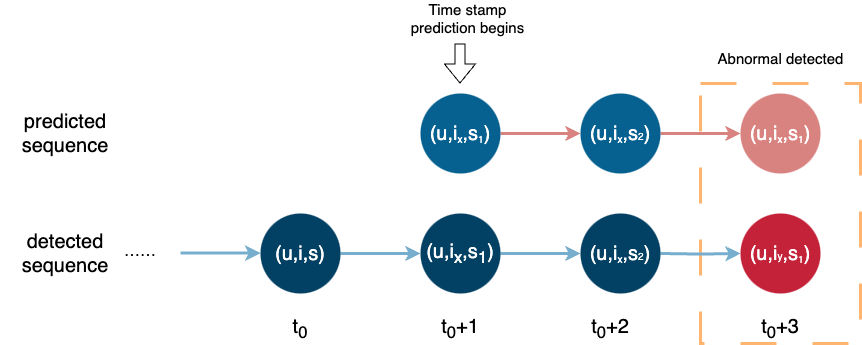
\includegraphics[width=\linewidth]{figures/04_anormal_detection.png}
    \caption{Abnormal Detection Process}
    \label{fig:anormal_detection}
\end{figure}

Suppose the vehicle equipped with our model also has a camera to film the driver's behavior. The video will be processed to generate the dynamic graph, and the model will predict the behavior state of the driver.
Starting at the point when the prediction begins, a comparison will take place in each timestamp afterwords. Once the predicted behavior state is different from the actual behavior state, the model will draw attention to it immediately. Once this anomaly accumulates to some threshold, the model will alert the driver or the system to take action. 
